% Transcripción fiel de paper_cacic_LNCS_word.docx.
% NO corregir ni actualizar nada: este árbol es la línea de base de
% trazabilidad contra la que se compara paper/02_reescrito/.
\documentclass[runningheads]{llncs}
\usepackage[T1]{fontenc}
\usepackage[utf8]{inputenc}
\usepackage[spanish,es-tabla,es-noquoting]{babel}
\usepackage{graphicx}
\usepackage{booktabs}

\begin{document}

\title{Modelos de Lenguaje Pequeños para la Interpretación de Comandos de
Domótica en Español: Un Estudio Comparativo}
\author{[Nombre y Apellido del autor/a]}
\institute{[Afiliación / Institución]\\ \email{[correo@institucion.edu.ar]}}
\maketitle

\begin{abstract}
Los asistentes de domótica basados en modelos de lenguaje suelen depender de
servicios en la nube, lo que introduce alta latencia, costos recurrentes y
dependencia de conectividad. Los Small Language Models (SLMs) ejecutados
localmente son una alternativa atractiva para hubs domóticos de bajo costo,
pero su capacidad real para interpretar comandos de voz en español
rioplatense no ha sido evaluada en profundidad. Este trabajo presenta un
dataset de 32 comandos de domótica en español, con anotaciones de referencia
(intención, dispositivo, ubicación, valor y unidad), y una evaluación
empírica de cuatro SLMs open-source (SmolLM2-360M-Instruct,
Qwen2.5-0.5B-Instruct, Qwen2.5-1.5B-Instruct y SmolLM2-1.7B-Instruct)
ejecutados en CPU con decodificación determinista. Los resultados muestran
una mejora consistente de la coincidencia exacta con el tamaño del modelo
(18,8\% a 59,4\%), a costa de un crecimiento de casi 4x en la latencia de
inferencia (15,6s a 61,9s por comando). La exactitud por campo revela que la
interpretación de valores y unidades numéricas se estanca entre 75\% y 90\%
independientemente del tamaño, y que los cuatro modelos fallan
sistemáticamente (0\%-17\% de exactitud) al interpretar comandos con ajustes
relativos o cualitativos sin un valor explícito, tendiendo a alucinar un
valor o unidad inexistente en el comando original.

\keywords{modelos de lenguaje pequeños, domótica, procesamiento del lenguaje
natural, interpretación de intención, computación en el borde, español
rioplatense.}
\end{abstract}

\section{Introducción}

El crecimiento de los asistentes de voz y los sistemas domóticos ha
popularizado el uso de modelos de lenguaje para interpretar comandos en
lenguaje natural (``prendé la luz del living'', ``bajá el aire a 20
grados''). La mayoría de las soluciones comerciales dependen de modelos de
gran escala alojados en la nube, lo que introduce tres problemas recurrentes
en el contexto de un hogar: latencia de red, costo recurrente por uso de
API, y dependencia de conectividad — un comando tan simple como apagar una
luz no debería fallar por una caída de internet.

Una alternativa creciente es el uso de Small Language Models (SLMs) —
modelos de lenguaje de entre unos cientos de millones y pocos miles de
millones de parámetros — ejecutados localmente en el propio hub domótico
(una Raspberry Pi, un mini-PC o un microcontrolador de gama alta). Trabajos
recientes muestran que estos modelos pueden alcanzar, en tareas acotadas, un
desempeño competitivo frente a modelos mucho más grandes \cite{gupta2025slms}.
Sin embargo, la mayor parte de la literatura sobre SLMs y asistentes
domóticos evalúa el inglés, y no está claro cómo se comportan estos modelos
frente a estructuras propias del español rioplatense (voseo, diminutivos,
expresiones relativas como ``bajale un toque'') ni cuál es el costo real en
latencia de ejecutarlos en hardware modesto.

Este trabajo aborda esa brecha mediante un estudio comparativo controlado.
Las contribuciones de este paper son: (1) un dataset de 32 comandos de
domótica en español rioplatense, organizados en seis categorías
lingüísticas, con una estructura de referencia (ground truth) de cinco
campos; (2) una evaluación empírica de cuatro SLMs open-source —
SmolLM2-360M-Instruct, Qwen2.5-0.5B-Instruct, Qwen2.5-1.5B-Instruct y
SmolLM2-1.7B-Instruct — ejecutados en CPU, midiendo coincidencia exacta,
exactitud por campo, validez del formato de salida y latencia; y (3) un
análisis cualitativo de los patrones de error que identifica una debilidad
sistemática, independiente del tamaño del modelo, en la interpretación de
comandos relativos o cualitativos sin valor numérico explícito.

\section{Trabajos relacionados}

La tarea de convertir un comando en lenguaje natural en una estructura de
intención y argumentos (slots) tiene una larga tradición en Natural Language
Understanding (NLU). Weld et al. \cite{weld2023survey} relevan en detalle
los modelos conjuntos de detección de intención y slot filling previos a la
era de los LLMs, basados típicamente en arquitecturas recurrentes o
transformers entrenados específicamente para el dominio; ese marco es el
punto de comparación natural para el enfoque, cada vez más común, de
resolver la misma tarea mediante la generación directa de una estructura
(JSON) con un modelo de lenguaje general o pequeño, sin entrenamiento
específico de slots.

En cuanto a corpus específicos de domótica, Bouraoui et al.
\cite{bouraoui2018french} construyeron y evaluaron un corpus de comandos de
voz para hogar inteligente en francés, mostrando que los recursos de NLU
para asistentes domóticos en inglés no transfieren bien a otros idiomas y
que las particularidades léxicas y sintácticas de cada lengua requieren
corpus propios. El presente trabajo sigue una lógica similar para el
español rioplatense, aunque a escala más acotada (un dataset de evaluación,
no de entrenamiento).

El antecedente más cercano a este trabajo es el estudio sobre LLMs
on-device para home assistants \cite{ondevice2025homeassistant}, que evalúa
variantes cuantizadas (16-bit, 8-bit y 4-bit) de modelos locales en un doble
rol de detección de intención y generación de respuesta, reportando entre
80\% y 86\% de exactitud sobre prompts no sintéticos y latencias de 5 a 6
segundos por consulta en el hardware utilizado. Este trabajo se diferencia
en tres aspectos: explora el extremo inferior de tamaño de modelo (SLMs de
0,36B a 1,7B parámetros, sin cuantización agresiva), evalúa en español
rioplatense en lugar de inglés, y se concentra en la tarea de interpretación
estructurada (intent + slots) en lugar de la generación conversacional de
respuestas.

Finalmente, el survey de Lu et al. \cite{gupta2025slms} sobre SLMs mapea el
estado del arte de modelos como Qwen, Llama 3.2, Phi, Gemma y SmolLM2, y
documenta que modelos de pocos miles de millones de parámetros pueden
alcanzar paridad de tarea específica frente a modelos mucho más grandes
cuando se entrenan con datos de alta calidad, lo que motiva evaluarlos en
tareas acotadas y de alto valor práctico como la interpretación de comandos
domóticos. Los reportes técnicos de Qwen2.5 \cite{qwen2024report} y SmolLM2
\cite{allal2024smollm2} documentan las arquitecturas y el entrenamiento de
los cuatro modelos utilizados en este estudio.

Un aspecto metodológico relevante para este trabajo es la decodificación
restringida por gramática (grammar-constrained decoding), que fuerza al
modelo a generar únicamente tokens compatibles con un esquema JSON o una
gramática formal en cada paso, garantizando validez sintáctica
independientemente de la capacidad del modelo
\cite{beurerkellner2024guiding,dong2024xgrammar}. En este estudio se optó
deliberadamente por no usar decodificación restringida, para medir la
capacidad de seguimiento de instrucciones del modelo en un escenario de
despliegue simple (sólo prompting, sin infraestructura adicional). Esta
decisión metodológica es relevante para interpretar los resultados: las
técnicas de decodificación restringida resuelven la validez de formato,
pero no evitan que el modelo alucine un valor semánticamente incorrecto
dentro de una estructura JSON perfectamente válida — que es precisamente el
problema central identificado en la Sección 4.4. Dicho de otro modo, el
100\% de JSON válido obtenido por los cuatro modelos (Tabla 2) no habría
sido garantía de exactitud semántica aun si se hubiese forzado
sintácticamente, lo que separa con claridad estos dos ejes de evaluación.

\section{Metodología}

\subsection{Modelos evaluados}

Se seleccionaron cuatro modelos open-source, sin restricciones de licencia
para descarga (no gated), cubriendo un rango de tamaño de 0,36 a 1,71 mil
millones de parámetros (Tabla 1).

\begin{table}[htbp]
\centering
\caption{Modelos evaluados en este estudio.}
\label{tab:orig-modelos}
\begin{tabular}{lll}
\toprule
Modelo & Parámetros & Familia / origen \\
\midrule
SmolLM2-360M-Instruct & 0.36 B & HuggingFaceTB \\
Qwen2.5-0.5B-Instruct  & 0.49 B & Alibaba (Qwen) \\
Qwen2.5-1.5B-Instruct  & 1.54 B & Alibaba (Qwen) \\
SmolLM2-1.7B-Instruct  & 1.71 B & HuggingFaceTB \\
\bottomrule
\end{tabular}
\end{table}

Todos los modelos se ejecutaron con la librería transformers, en precisión
bfloat16 y sin cuantización adicional, sobre una máquina virtual con 2
núcleos de CPU y 7,8 GB de RAM, sin aceleración por GPU. La decodificación
fue determinista (greedy, sin muestreo, temperatura no aplicada) para
aislar la variable de tamaño del modelo del efecto de la aleatoriedad y
garantizar reproducibilidad.

\subsection{Dataset de comandos}

Se diseñó manualmente un conjunto de 32 comandos de domótica en español
rioplatense (voseo), organizado en seis categorías que capturan distintos
desafíos lingüísticos: encendido/apagado simple, ajuste con valor numérico
explícito (grados o porcentaje), ajuste relativo o cualitativo sin valor
numérico (``bajale un poco''), comandos sobre múltiples dispositivos
(``todas las luces''), consultas de estado, y comandos con contexto
conversacional o negación. Cada comando cuenta con una anotación de
referencia (ground truth) de cinco campos: intent (encender / apagar /
ajustar / consultar), dispositivo, ubicación, valor y unidad.

\subsection{Protocolo de prompting y esquema de salida}

Se utilizó un único prompt de sistema, idéntico para los cuatro modelos, que
especifica el esquema JSON de salida, el vocabulario de dispositivos y
ubicaciones esperado, y dos ejemplos few-shot (no incluidos en el conjunto
de evaluación). Se instruyó a los modelos a responder únicamente con el
objeto JSON, sin texto adicional. El uso de un prompt idéntico para todos
los modelos privilegia la comparabilidad por sobre el desempeño máximo de
cada modelo individual: es posible que un prompt afinado por modelo mejore
los resultados de cada uno, pero a costa de introducir una variable de
confusión en la comparación.

\subsection{Métricas}

Se reportan cinco métricas: (1) tasa de JSON válido (respuesta parseable
como objeto JSON); (2) coincidencia exacta (los cinco campos coinciden con
el ground truth); (3) exactitud por campo (intent, dispositivo, ubicación,
valor, unidad evaluados individualmente); (4) latencia promedio de
inferencia por comando, en segundos, en el entorno de CPU descripto; y (5)
exactitud por categoría lingüística del comando.

\subsection{Prompt utilizado}

Para favorecer la reproducibilidad del estudio, se reproduce a continuación
una versión condensada del prompt de sistema (idéntico en su versión
completa para los cuatro modelos), que en la implementación real incluía
además un segundo ejemplo few-shot omitido aquí por espacio:

\begin{quote}
Sos un módulo de interpretación de comandos de voz para un sistema domótico
en español rioplatense. Convertí el comando del usuario en UN objeto JSON
con estos campos: ``intent'' (encender/apagar/ajustar/consultar),
``dispositivo'' (luz, aire\_acondicionado, calefaccion, persiana, cortina,
tv, parlante, cerradura, ventilador, todos), ``ubicacion'' (living, cocina,
dormitorio, bano, garage, patio, entrada, todas), ``valor'' (número si el
comando lo da, si no null), ``unidad'' (``\%'' o ``$^{\circ}$C'' si
corresponde, si no null). Reglas: respondé SOLO el JSON, sin texto
adicional; si el comando ajusta sin dar un número, ``valor'' y ``unidad''
deben ser null. Ejemplo: Comando: ``Poné el aire de la cocina en 20
grados.'' \{"intent": "ajustar", "dispositivo": "aire\_acondicionado",
"ubicacion": "cocina", "valor": 20, "unidad": "$^{\circ}$C"\}
\end{quote}

Cada comando de evaluación se envió como un turno de usuario adicional
(Comando: ``...'') inmediatamente después de este prompt de sistema, sin
turnos previos de conversación.

\section{Experimentación y resultados}

\subsection{Resultados globales}

La Tabla 2 resume los resultados agregados sobre los 32 comandos del
dataset. Los cuatro modelos alcanzaron 100\% de validez de formato JSON, lo
que indica que incluso el modelo más pequeño (360M parámetros) es capaz de
seguir instrucciones de formato estructurado de forma consistente en este
dominio acotado.

\begin{table}[htbp]
\centering
\caption{Resultados globales por modelo (n=32 comandos).}
\label{tab:orig-globales}
\begin{tabular}{lllll}
\toprule
Modelo & Parámetros & JSON válido & Coincidencia exacta & Latencia (s) \\
\midrule
SmolLM2-360M & 0.36B  & 100.0\% & 18.8\% & 15.6 \\
Qwen2.5-0.5B & 0.494B & 100.0\% & 43.8\% & 14.7 \\
Qwen2.5-1.5B & 1.54B  & 100.0\% & 50.0\% & 43.2 \\
SmolLM2-1.7B & 1.71B  & 100.0\% & 59.4\% & 61.9 \\
\bottomrule
\end{tabular}
\end{table}

\begin{figure}[htbp]
\centering
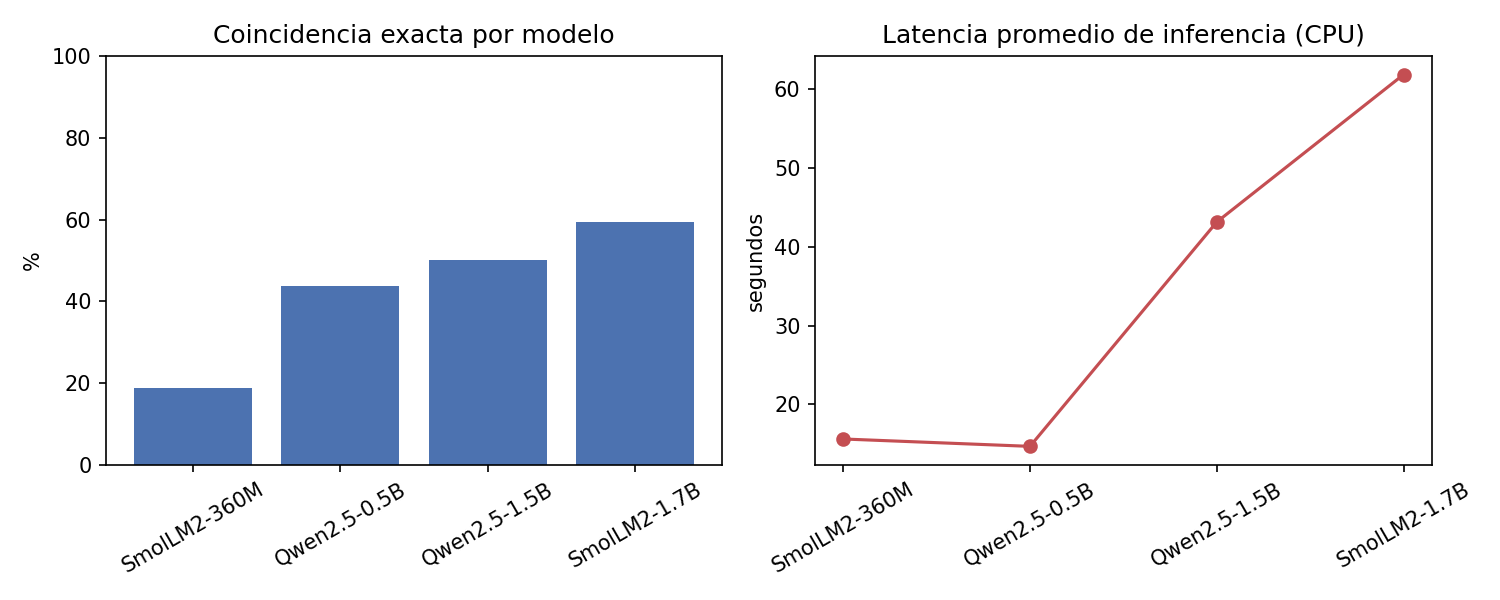
\includegraphics[width=\textwidth]{../../figures/fig1_exactitud_latencia.png}
\caption{Coincidencia exacta (izquierda) y latencia promedio de inferencia en
CPU (derecha), por modelo.}
\label{fig:orig-fig1}
\end{figure}

La coincidencia exacta crece de forma consistente con el tamaño del modelo
(18,8\% → 43,8\% → 50,0\% → 59,4\%), pero la latencia crece de forma mucho
más pronunciada: el modelo más grande (SmolLM2-1.7B) es casi 4 veces más
lento que el más chico (61,9s vs. 15,6s por comando), y llamativamente más
lento que Qwen2.5-1.5B (43,2s) a pesar de tener un 11\% más de parámetros —
una diferencia que probablemente responda a diferencias arquitectónicas o
de tokenizador entre familias, y no únicamente al conteo de parámetros.

\subsection{Exactitud por campo del esquema}

Descomponer la exactitud por campo (Fig. 2) muestra un patrón más matizado
que el de la coincidencia exacta agregada. Los campos intent, dispositivo y
ubicación mejoran de forma clara con el tamaño del modelo (intent: 40,6\% →
84,4\% → 93,8\% → 87,5\%; ubicación: 71,9\% → 81,2\% → 90,6\% → 96,9\%). En
cambio, los campos valor y unidad se mantienen relativamente estancados
entre 75\% y 90\% en los cuatro modelos, sin una tendencia monótona clara —
el modelo más grande (SmolLM2-1.7B) no supera a Qwen2.5-1.5B en ninguno de
estos dos campos.

\begin{figure}[htbp]
\centering
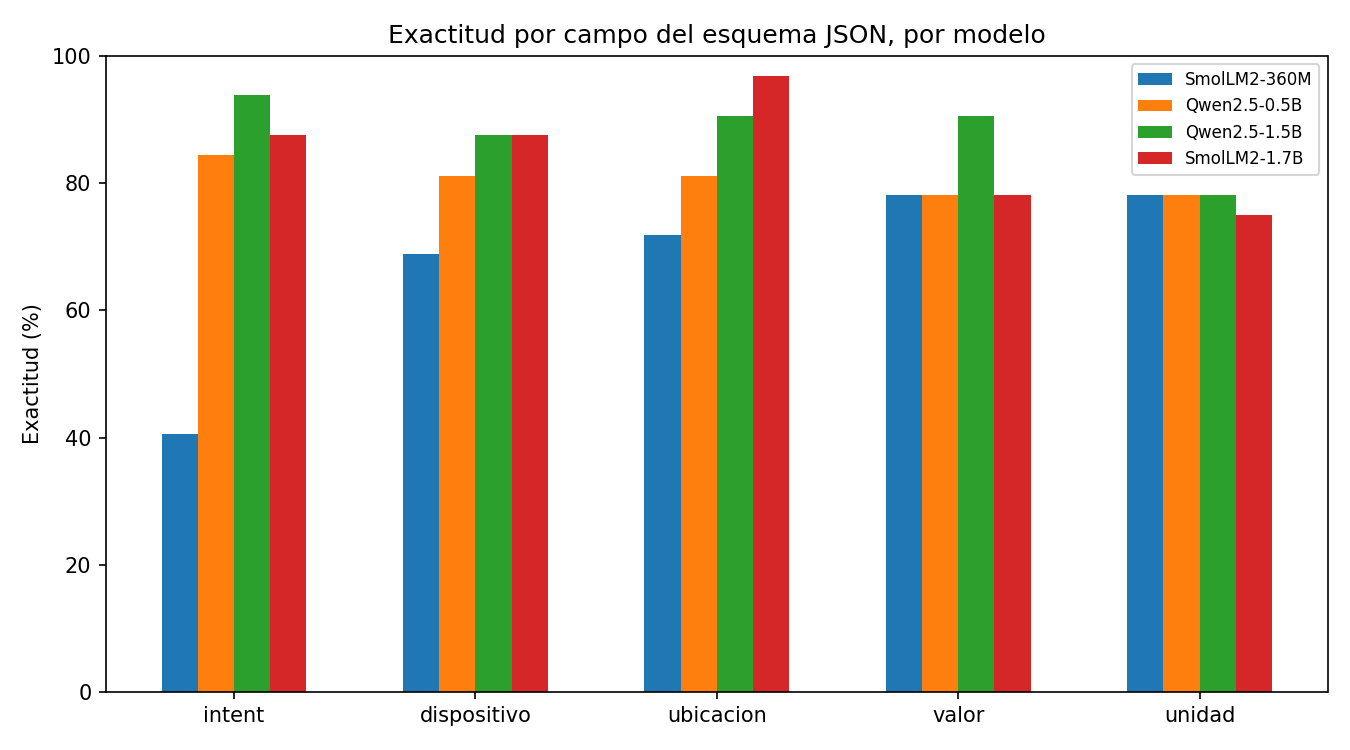
\includegraphics[width=\textwidth]{../../figures/fig2_exactitud_por_campo.png}
\caption{Exactitud por campo del esquema JSON (intención, dispositivo,
ubicación, valor, unidad), por modelo.}
\label{fig:orig-fig2}
\end{figure}

\subsection{Exactitud por categoría de comando}

La Tabla 3 desagrega la coincidencia exacta por categoría lingüística. Las
columnas de modelo se abrevian por su cantidad de parámetros (360M, 0.5B,
1.5B, 1.7B), en el mismo orden que la Tabla 2. La categoría de ajustes
relativos o cualitativos sin valor numérico explícito (por ejemplo,
``bajale un poco a la luz del living'') es, por lejos, la más difícil para
los cuatro modelos, con una exactitud de apenas 0\% a 16,7\% incluso en el
modelo más grande evaluado. Es importante notar que las categorías de
consulta de estado y negación/contexto tienen sólo 3 comandos cada una, por
lo que sus porcentajes deben leerse con cautela (representan 1 o 2 aciertos
sobre 3 casos).

\begin{table}[htbp]
\centering
\caption{Coincidencia exacta por categoría lingüística de comando y modelo.}
\label{tab:orig-categorias}
\begin{tabular}{lllll}
\toprule
Categoría (n) & 360M & 0.5B & 1.5B & 1.7B \\
\midrule
Encendido / apagado simple (n=8)           & 12.5\% & 62.5\% & 62.5\% & 75.0\% \\
Ajuste con valor numérico (n=8)            & 25.0\% & 75.0\% & 87.5\% & 87.5\% \\
Ajuste relativo / cualitativo (n=6)        & 0.0\%  & 0.0\%  & 16.7\% & 16.7\% \\
Múltiples dispositivos (n=4)               & 0.0\%  & 25.0\% & 25.0\% & 50.0\% \\
Consulta de estado (n=3)                   & 66.7\% & 33.3\% & 33.3\% & 33.3\% \\
Negación / contexto conversacional (n=3)   & 33.3\% & 33.3\% & 33.3\% & 66.7\% \\
\bottomrule
\end{tabular}
\end{table}

\subsection{Análisis cualitativo de errores}

Para caracterizar mejor la naturaleza de los errores más allá del
porcentaje agregado, se clasificó manualmente cada una de las 73 respuestas
incorrectas (sobre 128 corridas totales) en una o más de cuatro categorías
no excluyentes: confusión de intención (el campo intent no coincide),
confusión de dispositivo, confusión de ubicación, y alucinación de
valor/unidad (el modelo asigna un valor o unidad numérica cuando el ground
truth es null) o valor numérico incorrecto (cuando sí correspondía un
número pero el valor difiere). La Tabla 4 resume esta clasificación.

\begin{table}[htbp]
\centering
\caption{Taxonomía de errores por modelo (cantidad de casos por categoría,
sobre el total de respuestas incorrectas de cada modelo; un caso puede
pertenecer a más de una categoría).}
\label{tab:orig-taxonomia}
\begin{tabular}{lllll}
\toprule
Categoría de error & 360M & 0.5B & 1.5B & 1.7B \\
\midrule
Total de respuestas incorrectas & 26 & 18 & 16 & 13 \\
Confusión de intención          & 19 & 5  & 2  & 4  \\
Confusión de dispositivo        & 10 & 6  & 4  & 4  \\
Confusión de ubicación          & 9  & 6  & 3  & 1  \\
Alucinación de valor/unidad     & 0  & 5  & 7  & 7  \\
Valor numérico incorrecto       & 7  & 2  & 1  & 1  \\
\bottomrule
\end{tabular}
\end{table}

La taxonomía revela un desplazamiento cualitativo del error dominante a
medida que crece el modelo: en SmolLM2-360M, el 73\% de los errores (19 de
26) son confusión de intención, mientras que la alucinación de valor/unidad
es inexistente en ese modelo. En SmolLM2-1.7B ocurre lo opuesto: la
confusión de intención cae a 4 casos pero la alucinación de valor/unidad
pasa a ser, junto con la confusión de dispositivo, el error más frecuente
(7 de 13, 54\%) — consistente con la Sección 4.2: los modelos grandes
aprenden mejor qué intención y dispositivo corresponden, pero no a
abstenerse de completar un valor inexistente.

Un ejemplo particularmente ilustrativo es el comando ``Hace un poco más de
calor en el dormitorio, subí la calefacción'' (ground truth: valor=null,
unidad=null): SmolLM2-360M-Instruct confundió directamente la intención
(predijo ``consultar'' en lugar de ``ajustar''); Qwen2.5-0.5B-Instruct
predijo valor=15, unidad=``\%''; Qwen2.5-1.5B-Instruct predijo
unidad=``$^{\circ}$C'' (sin valor); y SmolLM2-1.7B-Instruct predijo valor=2,
unidad=``$^{\circ}$C''. Los cuatro modelos fallaron, pero de maneras
cualitativamente distintas — el más chico por no entender la intención, los
tres restantes por alucinar una cifra o unidad inexistente en el comando
original.

Un segundo hallazgo surgió al inspeccionar los errores de ``confusión de
dispositivo'': varios no son errores semánticos sino de vocabulario. Ante el
comando ``Che, la tele del living quedó prendida, apagala por favor''
(ground truth: dispositivo=``tv''), los cuatro modelos identificaron
correctamente intención, ubicación y ausencia de valor, pero usaron
sinónimos distintos: SmolLM2-360M y Qwen2.5-0.5B predijeron ``tele'',
Qwen2.5-1.5B predijo ``televisor'', y ninguno usó el token ``tv'' del
vocabulario del prompt. Bajo coincidencia exacta estos casos se contabilizan
como error, aunque semánticamente la interpretación es correcta — un punto
retomado como amenaza a la validez de constructo en la Sección 6.

\section{Discusión}

Los resultados sugieren dos conclusiones prácticas para el diseño de
asistentes domóticos locales. En primer lugar, el tamaño del modelo mejora
de forma clara la interpretación de qué dispositivo, qué acción y en qué
ubicación (intent, dispositivo, ubicación), pero el costo en latencia crece
más rápido que la ganancia en exactitud: pasar de Qwen2.5-0.5B a
SmolLM2-1.7B multiplica la latencia por algo más de 4 (14,7s → 61,9s) a
cambio de una mejora de 15,6 puntos porcentuales en coincidencia exacta
(43,8\% → 59,4\%). Para un hub domótico real, donde la experiencia de
usuario depende de una respuesta rápida, Qwen2.5-1.5B-Instruct ofrece el
mejor compromiso observado en este estudio: una coincidencia exacta similar
a la del modelo más grande (50,0\% vs. 59,4\%) con una latencia bastante
menor (43,2s vs. 61,9s), y la mejor exactitud de campo ``valor'' (90,6\%) de
los cuatro modelos.

En segundo lugar, y quizás más relevante, el estancamiento en los campos
valor/unidad y el desempeño uniformemente bajo en la categoría de ajustes
relativos indican que escalar el modelo dentro del rango evaluado (0,36B a
1,7B) no alcanza para resolver esta clase de comando. Esto tiene una
implicancia de diseño concreta: un sistema domótico real podría
beneficiarse de una capa de post-procesamiento basada en reglas (por
ejemplo, detectar la ausencia de un número en el comando original y forzar
valor=null y unidad=null en la salida del modelo) en lugar de depender de
que el modelo aprenda esta restricción únicamente a partir de mayor escala.

El resultado llamativo de que SmolLM2-360M-Instruct obtuvo la mayor
exactitud en la categoría de consulta de estado (66,7\% vs. 33,3\% en los
otros tres) es probablemente ruido estadístico dado el tamaño reducido de
esa categoría (n=3) y no debería interpretarse como que el modelo más chico
interpreta mejor las consultas; un dataset más amplio por categoría es
necesario para confirmar o descartar este patrón.

\section{Amenazas a la Validez}

\textbf{Validez de constructo.} La métrica principal (coincidencia exacta)
exige coincidencia textual estricta con el ground truth, lo que penaliza
por igual un error semántico real (confundir ``luz'' con
``aire\_acondicionado'') y una variación de vocabulario correcta (predecir
``tele'' en lugar de ``tv''), como se discutió en la Sección 4.4. La
exactitud reportada es una cota inferior de la capacidad semántica real:
una evaluación con normalización de sinónimos probablemente arrojaría
porcentajes más altos, sin cambiar el ordenamiento entre modelos ni el
hallazgo central sobre alucinación de valor/unidad.

\textbf{Validez interna.} La decodificación determinista (greedy) elimina
la variabilidad de muestreo, pero no garantiza resultados representativos
de un despliegue con temperatura mayor a cero. La latencia se midió en una
única VM compartida (2 núcleos, 7,8 GB de RAM); variaciones de carga del
sistema pudieron introducir ruido en los tiempos, aunque no en las métricas
de exactitud.

\textbf{Validez externa.} El dataset de 32 comandos es acotado (entre 3 y 8
por categoría), lo que limita la significancia estadística de las
comparaciones por categoría. Se usó un único prompt sin optimización por
modelo ni cuantización agresiva (4-bit/8-bit). La entrada fue siempre texto
limpio, sin ruido de reconocimiento de voz (ASR), y no se cubrieron
variantes dialectales más allá del rioplatense.

\textbf{Validez de conclusión.} Con 3 a 8 observaciones por categoría, las
diferencias porcentuales entre modelos (Tabla 3) son indicativas, no
estadísticamente significativas en sentido formal. El hallazgo más sólido —
la dificultad sistemática con ajustes relativos sin valor explícito — se
apoya en que el patrón se repite en los cuatro modelos, lo que reduce el
riesgo de que sea un artefacto muestral.

\section{Conclusiones y trabajo futuro}

Este trabajo presentó una comparación empírica de cuatro Small Language
Models open-source (0,36B a 1,7B parámetros) en la tarea de interpretar
comandos de domótica en español rioplatense, usando un dataset propio de
32 comandos anotados. Los resultados muestran que la coincidencia exacta
mejora de forma consistente con el tamaño del modelo (18,8\% a 59,4\%),
pero con una latencia que crece más rápido que la exactitud, y que los
cuatro modelos comparten una debilidad sistemática en la interpretación de
comandos con ajustes relativos o cualitativos sin valor numérico explícito,
tendiendo a alucinar valores y unidades inexistentes en el comando
original — un patrón que no se corrige con más escala dentro del rango
evaluado.

Como trabajo futuro se plantea: (1) ampliar el dataset con más comandos por
categoría y con voz real transcripta por ASR; (2) evaluar el efecto de la
cuantización agresiva (4-bit, 8-bit) sobre el trade-off exactitud/latencia
en el mismo hardware; (3) evaluar estrategias de mitigación del sesgo de
alucinación de valor/unidad, como post-procesamiento basado en reglas o
fine-tuning de dominio con ejemplos negativos explícitos; y (4) extender la
evaluación a comandos multi-turno con contexto de diálogo.

\section*{Declaración sobre el uso de IA}

En la elaboración de este trabajo se utilizaron herramientas de
inteligencia artificial generativa (Claude, Anthropic) en las siguientes
etapas: (i) asistencia en el diseño y curación del dataset de comandos de
domótica; (ii) desarrollo del código utilizado para ejecutar la evaluación
experimental de los cuatro modelos; (iii) redacción y edición del
manuscrito; y (iv) generación de las figuras y tablas de resultados. Los
resultados experimentales reportados corresponden a la ejecución real de
los modelos evaluados sobre el dataset descripto en la Sección 3.2. Los
autores revisaron, validaron y son responsables del contenido, el análisis
y las conclusiones presentadas en este trabajo. Esta transparencia es
consistente con marcos de buenas prácticas propuestos recientemente para la
divulgación del uso de agentes de IA en la investigación académica
\cite{torassa2025etica}.


\bibliographystyle{splncs03}
\bibliography{refs}

\end{document}
